\documentclass[a4paper]{article}
\usepackage[english]{babel}
\usepackage[utf8]{inputenc}

\usepackage{fullpage} % Package to use full page
\usepackage{parskip} % Package to tweak paragraph skipping
\usepackage{tikz} % Package for drawing
\usepackage{amsmath}
\usepackage{hyperref}
\usepackage{algorithm}
\usepackage{algpseudocode}
\usepackage[inline]{enumitem}

\title{Python Exercises}
\date{}

\begin{document}

\maketitle
\tableofcontents
\newpage

% @@@@@@@@@@@@@@@@@@@@@@@@@@@@@@@@@@@@@@@@@@@@@
% @@@@@@@@@@@@@@@@@@@@@@@@@@@@@@@@@@@@@@@@@@@@@
% BEGINNER 1
\section{Beginner}
% @@@@@@@@@@@@@@@@@@@@@@@@@@@@@@@@@@@@@@@@@@@@@
% @@@@@@@@@@@@@@@@@@@@@@@@@@@@@@@@@@@@@@@@@@@@@

% ---------------------------------------------
\subsection{Hi, guys!} \label{hi}
% ---------------------------------------------

Define a function called \texttt{greet}, which takes no argument and prints a random string by choosing a random greeting response from one of \{\textit{"Welcome :))"}, \textit{"Heyy!"}, \textit{"Sup bro!"}, \textit{"Ahoy!"}, \textit{"Howdy-doody"}, \textit{"Greetings and salutations!"}, \textit{"Yo!"}, \textit{"Hola!"}, \textit{"Konichiwa!"}, \textit{"There you are!"}, \textit{"Well well, look at you!"}, \textit{"Salute plurimam dicit. Si vales, bene est, ego valeo."}, \textit{"Valar morghulis"}. \}

\textbf{Hints:}
\begin{enumerate}
    \item \texttt{random.choice}
\end{enumerate}

%%%%%%%%%%%%%%%%%%%%%%%%%%%%%%%%%%%%%%%%%%%
%%%%%%%%%%%%%%%%%%%%%%%%%%%%%%%%%%%%%%%%%%%
% BEGINNER 2
%%%%%%%%%%%%%%%%%%%%%%%%%%%%%%%%%%%%%%%%%%%
%%%%%%%%%%%%%%%%%%%%%%%%%%%%%%%%%%%%%%%%%%%
\subsection{PrintPrint..Print \textit{n}\textit{n}..\textit{n} timestimes..times}
% ---------------------------------------------

Define a function called \texttt{print\_n\_times}, which takes two arguments, a string \verb|s| and an integer \verb|n|, and prints the string \verb|n| times, each on a separate line. If \texttt{n} is meaningless (negative, float etc.) or \texttt{s} is not string whatsoever, then call \texttt{greet} function from \ref{hi}.

\textbf{Hints:}
\begin{enumerate}
    \item If \texttt{greet} is far far away, \texttt{import} it.
\end{enumerate}

%%%%%%%%%%%%%%%%%%%%%%%%%%%%%%%%%%%%%%%%%%%
%%%%%%%%%%%%%%%%%%%%%%%%%%%%%%%%%%%%%%%%%%%
% BEGINNER 3
%%%%%%%%%%%%%%%%%%%%%%%%%%%%%%%%%%%%%%%%%%%
%%%%%%%%%%%%%%%%%%%%%%%%%%%%%%%%%%%%%%%%%%%
\subsection{How many minutes do we have today?}
Knowing when the day will over is always useful. Define a function called \texttt{get\_minutes\_left} that takes two integer arguments, one is the hour $0\leq \text{hour} \leq 23$ and the other is minute $0\leq \text{minute} \leq 59$. Check the boundaries with \texttt{assert}, and returns how many minutes left to the midnight?
\par
How many minutes left to the next day if the clock is 00.00?

% @@@@@@@@@@@@@@@@@@@@@@@@@@@@@@@@@@@@@@@@@@@@@
% @@@@@@@@@@@@@@@@@@@@@@@@@@@@@@@@@@@@@@@@@@@@@
\newpage
\section{Intermediate}
% @@@@@@@@@@@@@@@@@@@@@@@@@@@@@@@@@@@@@@@@@@@@@
% @@@@@@@@@@@@@@@@@@@@@@@@@@@@@@@@@@@@@@@@@@@@@
\subsection{Heads Tails Heads Tails Heads Tails}
% ---------------------------------------------

The coin flip experiment results in binomial distribution. The probability of getting exactly $k$ successes in $n$ trials is given by 

\begin{equation}
	{n\choose k}p^k(1 - p)^{n - k}
	\label{binomial_dist}
\end{equation}

where $p=0.5$ is the probability of success in one event (heads or tails) and

\begin{equation}
	{n\choose k} = \frac{n!}{k!(n - k)!}
	\label{n choose k}
\end{equation}

Define a function called \texttt{get\_coin\_flip\_prob} that takes $n$ and $k$ as arguments and returns the probability in Equation \ref{binomial_dist}.

\textbf{Hints:}
\begin{enumerate}
    \item \texttt{math.factorial}
\end{enumerate}

\subsubsection{Sample size matters}

Test your function by computing the probability of 51 tails out of 100 trials and 510 tails out of 1000 trials. Which one is more probable?

%%%%%%%%%%%%%%%%%%%%%%%%%%%%%%%%%%%%%%%%%%%
%%%%%%%%%%%%%%%%%%%%%%%%%%%%%%%%%%%%%%%%%%%
% INTERMEDIATE 2
%%%%%%%%%%%%%%%%%%%%%%%%%%%%%%%%%%%%%%%%%%%
%%%%%%%%%%%%%%%%%%%%%%%%%%%%%%%%%%%%%%%%%%%
\newpage
\subsection{Am I primal?}
% ---------------------------------------------

Write a function that checks given number is prime or not. If it is, print \textit{"Congrats! I am proud, you are prime."}; if not, print \textit{"Well, you are not primal, but highly evolved."}

\vspace{0.5cm}
\textbf{Hints:}
\begin{enumerate}
    \item Go up to square root.
\end{enumerate}

%%%%%%%%%%%%%%%%%%%%%%%%%%%%%%%%%%%%%%%%%%%
%%%%%%%%%%%%%%%%%%%%%%%%%%%%%%%%%%%%%%%%%%%
% INTERMEDIATE 3
%%%%%%%%%%%%%%%%%%%%%%%%%%%%%%%%%%%%%%%%%%%
%%%%%%%%%%%%%%%%%%%%%%%%%%%%%%%%%%%%%%%%%%%
\newpage
\subsection{Long live Euclid!}
Euclid’ s algorithm is a method for finding the greatest common divisor (GCD) of two numbers. Recall that the GCD of two numbers \verb|m| and \verb|n| is the largest number that divides both m and n.

\begin{algorithm}
    \caption{Division method}
    \begin{algorithmic}[1]
        \Function{gcd}{a, b}
            \While { b $ \neq $ 0 }
                \State temp = b
                \State b = a $ mod $ b
                \State a = temp
            \EndWhile
            \State \Return a
        \EndFunction
    \end{algorithmic}
\end{algorithm}

\begin{algorithm}
    \caption{Subtraction method}
    \begin{algorithmic}[1]
        \Function{gcd}{a, b}
            \While { a $ \neq $ b }
                \If {a $ > $ b}
                    \State a = a - b
                \Else
                    \State b = b - a
                \EndIf
            \EndWhile
            \State \Return a
        \EndFunction
    \end{algorithmic}
\end{algorithm}


\begin{algorithm}
    \caption{Recursive method}
    \begin{algorithmic}[1]
        \Function{gcd}{a, b}
            \If {b $ = $ 0}
                \State \Return a
            \Else
                \State \Return GCD(b, a $ mod $ b)
            \EndIf
        \EndFunction
    \end{algorithmic}
\end{algorithm}

\subsubsection{Divide, subtract and recurse} Implement all three versions above which takes
two integers as its arguments and returns their GCD. You may assume that both
inputs are integers, so there is no need to include any error checking in your function.

\subsubsection{Dare testing Euclid?} Test your functions for following pairs and compare functions to their running times.

\begin{itemize}
    \item 13, 13
    \item 20, 10
    \item 2017, 2018
    \item 5040, 60
    \item 73, 37
\end{itemize}

%%%%%%%%%%%%%%%%%%%%%%%%%%%%%%%%%%%%%%%%%%%
%%%%%%%%%%%%%%%%%%%%%%%%%%%%%%%%%%%%%%%%%%%
% INTERMEDIATE 4
%%%%%%%%%%%%%%%%%%%%%%%%%%%%%%%%%%%%%%%%%%%
%%%%%%%%%%%%%%%%%%%%%%%%%%%%%%%%%%%%%%%%%%%
\newpage
\subsection{Rohan had come at last}
\textit{In rode the Lord of the Nazgûl. \\
A great black shape against the fires beyond he loomed up, grown to a vast menace of despair. \\
In rode the Lord of the Nazgûl, under the archway that no enemy ever yet had passed, and all fled before his face. \\
All save one. There waiting, silent and still in the space before the Gate, sat Gandalf upon Shadowfax: \\
Shadowfax who alone among the free horses of the earth endured the terror, \\
unmoving, steadfast as a graven image in Rath Dínen. \\
"You cannot enter here," said Gandalf, and the huge shadow halted. \\
"Go back to the abyss prepared for you! Go back! Fall into the nothingness that awaits you and your Master. Go!" \\
The Black Rider flung back his hood, and behold! he had a kingly crown; and yet upon no head visible was it set. \\
The red fires shone between it and the mantled shoulders vast and dark. \\
From a mouth unseen there came a deadly laughter. "Old fool!" he said. \\
"Old fool! This is my hour. Do you not know Death when you see it? Die now and curse in vain!" \\ And with that he lifted high his sword and flames ran down the blade. \\
And in that very moment, away behind in some courtyard of the city, a cock crowed. \\
Shrill and clear he crowed, recking nothing of war nor of wizardry, \\
welcoming only the morning that in the sky far above the shadows of death was coming with the dawn. \\
And as if in answer there came from far away another note. \\
Horns, horns, horns, in dark Mindolluin's sides they dimly echoed. \\
Great horns of the north wildly blowing. Rohan had come at last.}

\subsubsection{Counting 'is' good}
An \textbf{n-gram} is a sequence of items from a given sample of text. For a unigram, $n$ is equal to $1$. For a bigram $n$ is equal to 2. An n-gram can be at character level as well as word level. We will look at word level n-grams here.
\par
Extract the word-level unigram for the text above. Clean all punctuation, lowercase the words, and collect all the words.
\par
Count all the words. What is the count of word \textit{'is'}?

\textbf{Hints:}
\begin{enumerate}
    \item \texttt{string.punctuation}
    \item \texttt{collections.Counter}
\end{enumerate}

\subsubsection{Oh my Lord}
Extract the word-level bigram of the text, namely, the list of each two adjacent words.
\par
Count all the pairs. What is the count of the phrase \textit{'the lord'}?

%%%%%%%%%%%%%%%%%%%%%%%%%%%%%%%%%%%%%%%%%%%
%%%%%%%%%%%%%%%%%%%%%%%%%%%%%%%%%%%%%%%%%%%
% INTERMEDIATE 5
%%%%%%%%%%%%%%%%%%%%%%%%%%%%%%%%%%%%%%%%%%%
%%%%%%%%%%%%%%%%%%%%%%%%%%%%%%%%%%%%%%%%%%%
\newpage
\subsection{B$e$hold, $e$ul$e$r!}
% ---------------------------------------------

The base of the natural logarithm, $e$, can be defined as the infinite sum (Taylor expansion)
\begin{equation}
	e = \sum_{k=0}^{\infty}\frac{1}{k!} = 1 + 1 + \frac{1}{2} + \frac{1}{6} + \frac{1}{24} + \dots
	\label{e_sum}
\end{equation}

But earlier (18th century), Bernoulli defined the compound interest problem

\begin{equation}
    \lim_{x \to \infty} \left(1 + \frac{1}{x}\right)^x
    \label{compound}
\end{equation}

Suppose you have a money in the bank. And the bank compounds the money annually. Equation \ref{compound} gives the increase rate of money if $100\%$ interest is compounded in one year where $x$ defines the number of the time that interest is applied. If $x=1$, $100\%$ interest is applied only at the end of the year. Then total rate becomes $2$, namely money is doubled. If $x=2$, $50\%$ interest is applied twice through one year. In this case, total rate becomes $2.25$. What happens when $x \to \infty$ as in the Equation \ref{compound}? This is where Euler comes in. He calculated this converging sum and ended up an irrational number $e=2.718281...$

\subsubsection{Comput$e$ $\lim_{x \to \infty} {1 + \frac{1}{x}}^x$ ul$e$r}
Define a function called \texttt{euler\_limit} that takes number $n$ and approximates Equation \ref{compound}. You may assume that the input to your function will be a positive integer.

\subsubsection{Comput$e$ $\sum_{k=0}^{\infty}\frac{1}{k!}$ ul$e$r}
Define a function called \texttt{euler\_infinite\_sum} that takes a non-negative integer argument $n$, and returns an approximation to $e$ based on the first $n$ terms of Equation \ref{e_sum}.

\textbf{Hints:}
\begin{enumerate}
    \item \texttt{euler\_infinite\_sum(0)} should give $0$.
\end{enumerate}

\subsubsection{Get to know $\epsilon$ul$e$r?}
Define a function called \texttt{euler\_approx} that takes an argument, a float \textit{epsilon}, and uses the sum in Equation \ref{e_sum} for an approximation of $e$ that is within \textit{epsilon} of the true value of $e$. 

\textbf{Hints:}
\begin{enumerate}
    \item \texttt{math.e}
\end{enumerate}

\subsubsection{Say his name r$e$p$e$at$e$dly!}
Define a function called \texttt{print\_euler\_sum\_table} that takes a positive integer $n$ as an argument and prints the successive values obtained from \texttt{euler\_infinite\_sum(k)} as $k$ ranges from $1$ to $n$, one per line.


% @@@@@@@@@@@@@@@@@@@@@@@@@@@@@@@@@@@@@@@@@@@@@
% @@@@@@@@@@@@@@@@@@@@@@@@@@@@@@@@@@@@@@@@@@@@@
% @@@@@@@@@@@@@@@@@@@@@@@@@@@@@@@@@@@@@@@@@@@@@
\newpage
\section{Advanced}
% @@@@@@@@@@@@@@@@@@@@@@@@@@@@@@@@@@@@@@@@@@@@@
% @@@@@@@@@@@@@@@@@@@@@@@@@@@@@@@@@@@@@@@@@@@@@
% @@@@@@@@@@@@@@@@@@@@@@@@@@@@@@@@@@@@@@@@@@@@@
\subsection{A Story of Creation}

\subsubsection{What are Gods? Immortal Men.}

\textit{In the beginning, there was only Chaos. No space, no time just endless Chaos. But Chaos was made of two siblings: the darkness (Erebus) and the night (Nyx). Their love gave birth to the Mother Earth, Gaia. And Gaia gave birth to the Father Sky, Uranus to equally cover herself. Then from their love 6 Titans, 6 Titanesses, one-eyed Cyclopses and hundred-arms Hecatoncheires were born. Titans ruled the Universe for a very long time.\\
Neither Father Uranus did not love his children nor the children did not love him back. He imprisoned them in Tartarus deep within the Earth where they gave pain to Gaia. She incited a riot among her children. One of the children, Cronus was willing to help his mother. He castrated Uranus and threw his testicles into the sea from which Aphrodite, the Goddess of Love was emerged.\\
New ruler, Cronus and his sister Rhea gave birth to the Hestia, Demeter, Hera, Hades, Poseidon and Zeus. Cronus thought that Zeus would be an opponent against him so he wanted to eat Zeus up. Rhea deceived Cronus by giving him a stone wrapped in baby's clothes.\\
After years, Gods have declared a war against the Titans. Gods have prevailed. Poseidon, Hades and Zeus possessed the Sea, the Underworld and the Sky respectively and sat on the throne in Mount Olympus. The Age of Gods had begun.}

Define an \texttt{Immortal} class with following attributes: \texttt{name, gender, essence}.

\begin{itemize}
    \item \texttt{name} : String. Name of the immortal.
    \item \texttt{gender} : String. Gender of the immortal. \texttt{female} or \texttt{male}.
    \item \texttt{essence} : String. Origin of the immortal. e.g. \textit{Sky} for \textit{the God of Sky}.
\end{itemize}

Write an initializer method that takes \texttt{name, gender, essence}. Immortals are binary(!) (\texttt{gender} must be \texttt{female} or \texttt{male}). Check if gender is given correctly.

\textbf{Hints:}
\begin{enumerate}
    \item \texttt{assert}
\end{enumerate}

\subsubsection{Immortals, how should I \textit{call} you?}

Define two classes that inherit from \texttt{Immortal}: \texttt{Titan} and \texttt{God}. Both have attributes \texttt{name, gender, essence}. Write printing methods for both \texttt{Titan} and \texttt{God} to see the name and essence when you print it. e.g. \textit{"Apollo, the God of Sun"}, \textit{"Athena, the Goddess of Wisdom"}, \textit{"Gaia, the Titaness of Earth"}.

\textbf{Hints:}
\begin{enumerate}
    \item \texttt{\_\_str\_\_} or \texttt{\_\_repr\_\_}
    \item Mind the gender!
    \item Name and essence are titled.
\end{enumerate}

\subsubsection{What are Men? Mortal Gods.}

\textit{...Titans were imprisoned in the eternal hell of Tartarus. But two Titans, Prometheus and Epimetheus stood by the side of the Gods. Zeus honored them with the task of creating all living things on Earth. Epimetheus gave the creatures a portion of Gods' abilities. Some had the ability to swim, to fly or to run fast. Some had thick furs and sharp claws for hunting. Meanwhile, Prometheus created humans with a great effort and gave them a reflection of the image of Gods. Zeus worried of seeing their reflections from above. He warned Prometheus that Humans must remain mortal and worship the Gods themselves. Although humans have specialized in many areas like craft, art, philosophy, science, they were in need of protection and care of the Gods to stay alive on the wild Earth.}

Define a \texttt{Mortal} class with following attributes: \texttt{name, gender, profession}.

\begin{itemize}
    \item \texttt{name} : String. Name of the mortal.
    \item \texttt{gender} : String. Gender of the mortal.
    \item \texttt{profession} : Optional String. Default value is empty string. Profession of the mortal.
\end{itemize}

Write an initializer method that takes \texttt{name}, \texttt{gender} and optional \texttt{profession}. Mortals are free in genders. (Any type of gender is acceptable, no need \texttt{Assertion}).

Define classes that inherit from \texttt{Mortal}: \texttt{Human} and \texttt{Creature}. All have attributes \texttt{name, gender, profession}. Write a printing method for all to see the name and the profession of the mortal when you print it. e.g. \textit{"Mortal man Achilles the Warrior"}, \textit{"Mortal man Homer the Author"}, \textit{"Mortal woman Hypatia the Mathematician"}, \textit{"Mortal creature Succubus the Seducer"}.

\subsubsection{Prometheus, show me how to \textit{burn}!}

\textit{...Prometheus was in agony to see his creations under oppression. He felt anger and vengeance against Zeus. So he presented less valuable parts of the meat of sacrifices made by Humans to the Gods. This made Zeus mad. He forbade the use of Fire on Earth to cook the meat or for any other purposes.\\
But Prometheus could not bear that his creations were unable to use this power. He climbed to Mount Olympus where the Fire was hidden inside the forge of Hephaestus, the God of Fire. He carried it down to the Humans. This power released the potential of Human mind and imagination. Hereafter, humans were able to harness nature, obtain better food resources and forge weapons. Civilization progress ramped up.\\
Zeus, the God of Gods were outraged when he saw all the lights spreaded around the Earth. He ordered that Prometheus was to be chained at the top of Mount Caucasus. A vulture would come daily to eat his liver which will be replenished at the end of the day. Prometheus was captured in an endless painful loop. However, he was at peace when looked at down below and see the sea of lights that illuminate his creations.}

Define \texttt{\_illumination} variable for only \texttt{Human} class at its initializer. Write \texttt{get} and \texttt{\_set} methods for it. Define \texttt{illuminate} method that calls \texttt{\_set} to increment \texttt{\_illumination}. All the changes defined below in detail should be in \texttt{Human} class. Remember, Humans got the Fire!

\begin{itemize}
    \item \texttt{\_illumination} : Private Integer. At initializer. Initial value is $1$ (A faint flame).
    \item \texttt{\_max\_illumination} : Private Integer. At initializer. Initial value is $1000$.
    \item \texttt{get\_illumination()} : Public method. Returns \texttt{\_illumination}.
    \item \texttt{\_set\_illumination(n)} : Private method. Sets \texttt{\_illumination} to \texttt{n}. Bound it between \\
          $[0, \texttt{\_max\_illumination}]$. (\textbf{Hint} : max() of min() or min() of max())
    \item \texttt{illuminate(delta)} : Public method. Increments \texttt{\_illumination} by \texttt{delta} calling\\
    \texttt{\_set\_illumination(n)} and \texttt{print} new \texttt{\_illumination} value e.g. \textit{Archimedes's illumination is 73}. Prevent exceeding \texttt{\_max\_illumination}.
\end{itemize}

\subsubsection{Eternal Fire, show me how to become Immortal!}

\textit{"What you leave behind is not what is engraved in stone monuments, but what is woven into the lives of others."} --- Pericles 

Define \texttt{influence\_range} for all classes that you have written. Define \texttt{influence(character)} method for both \texttt{Immortal} and \texttt{Mortal} classes. Define \texttt{\_become\_immortal()} method for only \texttt{Human} class. When \texttt{\_max\_illumination} is reached at \texttt{illuminate(delta)} method call \texttt{\_become\_immortal()}.

\begin{itemize}
    \item \texttt{influence\_range} : Public \texttt{range}. At initializer of all classes. Initial values are as follows:
    \begin{itemize}
        \item \texttt{range(-1, 2)} for \texttt{Immortal}
        \item \texttt{range(-1, 2)} for \texttt{Mortal}
        \item \texttt{range(-2, 7)} for \texttt{Titan}
        \item \texttt{range(-5, 9)} for \texttt{God}
        \item \texttt{range(-1, 11)} for \texttt{Human}
        \item \texttt{range(-3, 5)} for \texttt{Creature}
    \end{itemize}
    \item \texttt{influence(character)} : Public method. At only \texttt{Immortal} and \texttt{Mortal} classes. Takes a \texttt{Human} character, chooses random number \texttt{delta} in \texttt{influence\_range} and call \texttt{illuminate(delta)} method. (\textbf{Hint}: Check character type with \texttt{assert}.)
    \item \texttt{\_become\_immortal()} : Private method. At only \texttt{Human} class. First check if \texttt{\_illumination} reached to \texttt{\_max\_illumination}. Then change class type to \texttt{Immortal}, assign \texttt{profession} to \texttt{essence} and \texttt{print} new \texttt{self}. Call \texttt{\_become\_immortal()} method under \texttt{illuminate(delta)} method when \texttt{\_max\_illumination} is reached. (\textbf{Hints}: Use \texttt{\_\_class\_\_} to change class type. Assign \texttt{self.profession} to a variable before changing class type.)
\end{itemize}

\subsubsection{Ignite, burn and explode!}

\textit{...The Fire was spread on Earth at the hands of Humans who are blessed and guided by Prometheus, the Titan of Fire. One of the regions on Earth where the lights of Fire shine very bright was called Ionia.  Ionia's people held the Fire for generations and they harnessed the power of it to turned into knowledge and imagination. And some of the people were illuminated brightest among the mortals. So bright that meant to never fading fire which would be burning to the end of time, eternity. Their Fire guided all others who wanted to escape from darkness as once Prometheus guided them. They had become Immortals.}

Define a stand-alone function (not a part of any class) \texttt{spread\_the\_fire(influencers, flame\_holders)} as described below.

\begin{itemize}
    \item \texttt{influencers} : List of \texttt{Immortal} and \texttt{Mortal} instances.
    \item \texttt{flame\_holders} : List of \texttt{Immortal} and \texttt{Mortal} instances. 
    Both list should contain at least one \texttt{Human}. The best influencers for Humans are Humans themselves! (\textbf{Hint} : Check with \texttt{any} and \texttt{assert})
\end{itemize}

\begin{algorithm}
    \caption{\textit{Spreading the fire} algorithm}
    \begin{algorithmic}[1]
        \Function{Spread\_the\_Fire}{\texttt{influencers}, \texttt{flame\_holders}}
            \State \texttt{assert} \texttt{flame\_holders} contain at least one \texttt{Human}
            \State \texttt{assert} \texttt{influencers} contain at least one \texttt{Human}
            \While { \texttt{True} }
                \State Randomly choose one \texttt{influencer}
                \State Randomly choose one \texttt{flame\_holder}
                \State \texttt{try} influencing \texttt{flame\_holder}
                \If {\texttt{AssertionError} is caught}
                    \State \texttt{print} the error
                    \State \texttt{continue}
                \EndIf
                \If {\texttt{flame\_holder} became an \texttt{Immortal}}
                    \State \texttt{break}
                \EndIf
            \EndWhile
        \EndFunction
    \end{algorithmic}
\end{algorithm}

Some \texttt{Immortal} and \texttt{Mortal} instances you might want to use are as follows:

\begin{itemize*}
    \item \textit{Gaia, the Titaness of Earth}
    \item \textit{Uranus, the Titan of Sky}
    \item \textit{Chronus, the Titan of Harvest}
    \item \textit{Atlas, the Titan of Endurance}
    \item \textit{Prometheus, the Titan of Fire}\\

    \item \textit{Zeus, the God of Sky}
    \item \textit{Poseidon, the God of Sea}
    \item \textit{Hades, the God of Underworld}
    \item \textit{Apollo, the God of Sun}
    \item \textit{Athena, the Goddess of Wisdom}
    \item \textit{Dionysus, the Goddess of Wine}
    \item \textit{Aphrodite, the Goddess of Love}
    \item \textit{Ares, the God of War}
    \item \textit{Hera, the Goddess of Marriage}
    \item \textit{Artemis, the Goddess of Hunt}
    \item \textit{Demeter, the Goddess of Harvest}\\
    
    \item \textit{Mortal man Homeros the Author}
    \item \textit{Mortal man Thales the Philosopher}
    \item \textit{Mortal man Socrates the Philosopher}
    \item \textit{Mortal man Plato the Philosopher}
    \item \textit{Mortal man Aristotle the Philosopher}
    \item \textit{Mortal man Archimedes the Inventor}
    \item \textit{Mortal man Aristarchus the Astronomer}
    \item \textit{Mortal man Herodotus the Historian}
    \item \textit{Mortal woman Theano the Philosopher}
    \item \textit{Mortal man Sophocles the Poet}
    \item \textit{Mortal man Ictinus the Architect}
    \item \textit{Mortal man Phidias the Sculptor}
    \item \textit{Mortal woman Hypatia the Mathematician}\\
    
    \item \textit{Mortal gorgon Medusa the Monster}
    \item \textit{Mortal horse Pegasus the Flyer}
    \item \textit{Mortal hound Cerberus the Guard}
\end{itemize*}

Using the algorithm and sample characters described above, run\\ \texttt{spread\_the\_fire(influencers, flame\_holders)} and see who will be the first \texttt{Immortal}.\\
You can also define an \texttt{\_influencers} variable to see the most influent characters upon your \texttt{Immortal}.

\begin{itemize}
    \item \texttt{\_influencers} : Dictionary(\texttt{Immortal} or \texttt{Mortal}, Integer). Keys are influencer instance, values are their influence amount.
    \item \texttt{get\_influencers()} : Public method. Returns \texttt{\_influencers}.
    \item \texttt{\_set\_influencers(influencer, delta)} : Private method. Increments the value of \texttt{influencer} in \texttt{\_influencers} dictionary by \texttt{delta}.
\end{itemize}

\textbf{Hints:}
\begin{enumerate}
    \item Call \texttt{\_set\_influencers(influencer, delta)} in \texttt{Human} class. Do not call it from outside!
    \item Use \texttt{setdefault} to set default value of \texttt{\_influencers} dictionary.
    \item Get \texttt{influencer} object with \texttt{inspect.currentframe().f\_back.f\_locals['self']}
    \item \texttt{import inspect}
    \item Set new \texttt{influencers} dictionary for Mortals that became Immortals since you cannot reach \texttt{get\_influencers()} method.
\end{enumerate}

%%%%%%%%%%%%%%%%%%%%%%%%%%%%%%%%%%%%%%%%%%%
%%%%%%%%%%%%%%%%%%%%%%%%%%%%%%%%%%%%%%%%%%%
% ADVANCED 2
%%%%%%%%%%%%%%%%%%%%%%%%%%%%%%%%%%%%%%%%%%%
%%%%%%%%%%%%%%%%%%%%%%%%%%%%%%%%%%%%%%%%%%%
\newpage
\subsection{Again, $e$ul$e$r}

Euler method is used to solve ordinary differential equations (ODE)s.

General first order differential equation form is

\begin{equation}
	\frac{dy}{dt} = f(t, y), \hspace{1cm} y(t_0) = y_0
\end{equation}

We want to approximate the solution to (1) near $ t_0 $. We only know the value of the solution and its derivative at initial point. We can get this by plugging the initial condition into $ f(t, y) $ into the differential equation itself.  So, the derivative at this point is.

\begin{equation}
	\frac{dy}{dt}\Bigr|_{\substack{t=t_0}} = f(t_0, y_0) \approx \frac{y - y_0}{t - t_0}
\end{equation}

\begin{figure}[htbp]
    \begin{center}
        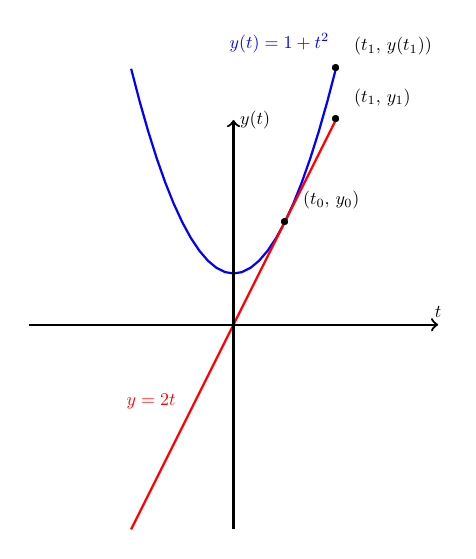
\begin{tikzpicture}[thick,scale=0.65, every node/.style={scale=0.65}]
        \draw[domain=-2:2, color=blue] plot (\x, {1 + (\x)^2}) node[above = .5cm, left, color=blue] {$y(t)=1 + t^2$};
        \draw[domain=-2:2, color=red] plot(\x,2 * \x) node[below=5.5cm, left=3.0cm, color=red] {$y=2t$};
        \draw [thick, ->] (-4,0) -- (4,0) node [above] {$t$};
        \draw [thick, ->] (0,-4) -- (0,4) node [right] {$y(t)$};
        \node [label={[label distance=0.01cm]30:($t_0$, $y_0$)}] at (1,2) {\textbullet};
        \node [label={[label distance=0.01cm]30:($t_1$, $y_1$)}] at (2,4) {\textbullet};
        \node [label={[label distance=0.01cm]30:($t_1$, $y(t_1)$)}] at (2,5) {\textbullet};
        \end{tikzpicture}
    \end{center}
    \caption{Sample approach for the plot of $f(x)=1+t^2$ with a tangent at $t_0=1.0$.}\label{eulerplot}
\end{figure}

In Fig. \ref{eulerplot}, if $ t_1 $ is close enough to $ t_0 $ then the point $ y_1 $ on the tangent line should be fairly close to the actual value of the solution at  $ t_1 $. Finding $ y_1 $ is easy enough. All we need to do is plug $ t_1 $ in the equation for the tangent line.

\begin{equation}
	y_1 = y_0 + f(t_0, y_0)(t_1 - t_0)
\end{equation}

This $ y_1 $ is only an approximation. If we accept the error, we can continue build up lines similarly.

\begin{equation}
	y_2 = y_1 + f(t_1, y_1)(t_2 - t_1)
\end{equation}

\begin{equation}
	y_3 = y_2 + f(t_2, y_2)(t_3 - t_2)
\end{equation}

In general, starting from the initial point, $ (t_n, y_n) $ we have an approximation at $ (t_{n + 1}, y_{n + 1}) $ like

\begin{equation}
	y_{n + 1} = y_n + f(t_n, y_n)(t_{n + 1} - t_n)
\end{equation}

If we were to take a constant step size

\begin{equation}
	t_{n + 1} - t_n = h
\end{equation}

Equation (6) would be,

\begin{equation}
	y_{n + 1} = y_n + h.f(t_n, y_n)
\end{equation}

But of course this step size may not be constant, but adaptive.

We start at initial point $ (t_0, y_0) $ and repeatedly evaluate new points with selected or adaptive step size. We continue until we reach the target point that we want to compute (We will acquire $ y(t_f) $ for target point $ t_f $).

\begin{figure}[ht]
	\centering
    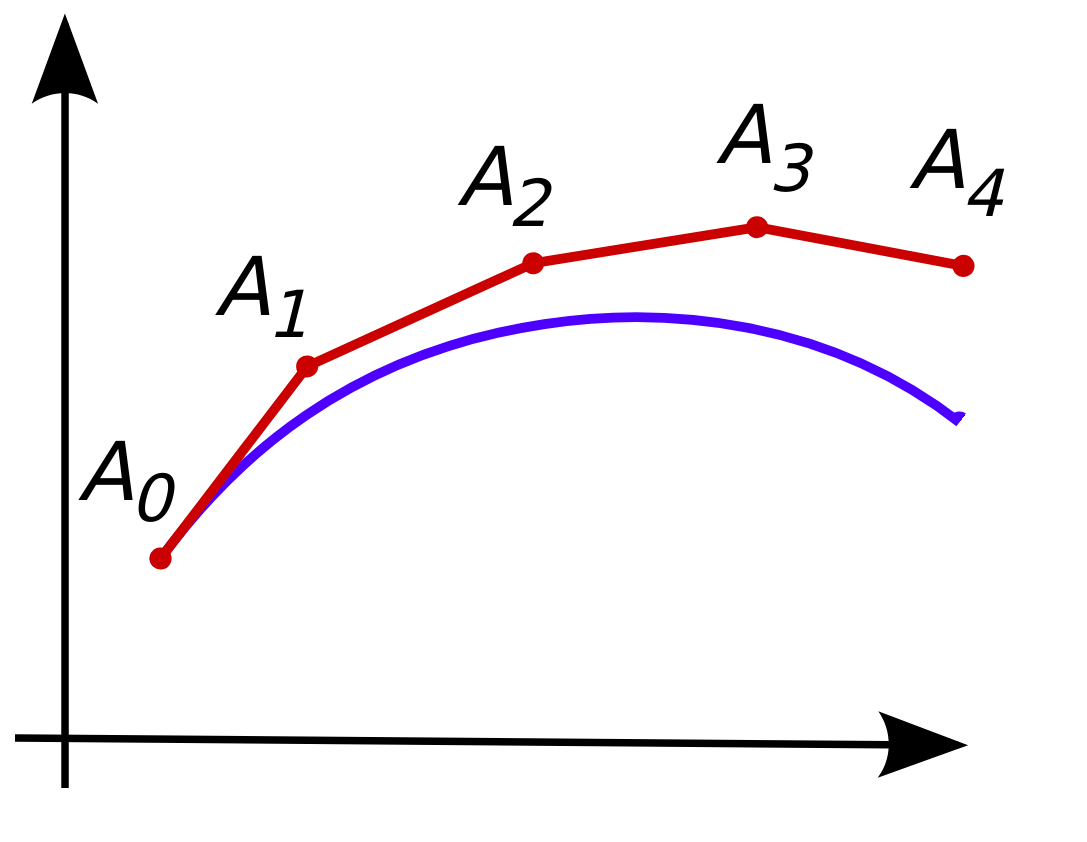
\includegraphics[scale=0.2]{euler.png}
    \label{euler}
    \caption{Euler approximation steps}
\end{figure}

Here is a pseudo-code for algorithm where $n$ is the number of steps.

\begin{algorithm}
    \caption{Euler method with constant step size}
    \begin{algorithmic}[1]
        \Function{Euler}{$f, t_0, y_0, n, t_f$}
            \State Compute step size $h$
            \For{$i$ from $1$ to $n$}
                \State Compute $f(t_0, y_0)$
                \State Compute new $t_1$
                \State Compute corresponding $y_1$
                \State Update $t_0$ and $y_0$
            \EndFor
            \State \Return $y_0$
        \EndFunction
    \end{algorithmic}
\end{algorithm}

\subsubsection{Pati$e$nc$e$! St$e$p by st$e$p}
Write a function that takes function $ f $, initial points $ t_0 $ and $ y_0 $, number of steps $ n $ and target point $ t_f $ and returns approximate $ y_f $ value.

\subsubsection{Dar$e$ to t$e$st $e$ul$e$r?}
Test your function for following differential equations with given initial points at desired target points with different number of steps $ n $. Compare your results to given analytic solutions. Show your numerical results and analytic results and their relative errors for different $ n $' s.

\begin{align*}
    i) \hspace{0.5cm} \frac{dy}{dt} = y + t \hspace{0.5cm} y(0) = 0 \hspace{2cm}  
    \textbf{analytic solution:} (y = e^t - t -1)
\end{align*}

\begin{align*}
    ii) \hspace{0.5cm} \frac{dy}{dt} = \sin{t} - \frac{y}{t} \hspace{0.5cm} y(0) = 0 \hspace{2cm}  
    \textbf{analytic solution:} (y = \frac{\sin{t}}{t} - \cos{t})
\end{align*}

% \subsection{Question c)}
% Write same method with adaptive step size, instead of constant step size and compare with previous approach.

\vspace{1cm}
\textbf{Hints:}
\begin{enumerate}
    \item Use only \verb|math| library.
    \item $ \text{relative error} = \frac{|\text{predicted value} - 
            \text{true value}|}{\text{true value}} $
\end{enumerate}

%%%%%%%%%%%%%%%%%%%%%%%%%%%%%%%%%%%%%%%%%%%
%%%%%%%%%%%%%%%%%%%%%%%%%%%%%%%%%%%%%%%%%%%
% ADVANCED 3
%%%%%%%%%%%%%%%%%%%%%%%%%%%%%%%%%%%%%%%%%%%
%%%%%%%%%%%%%%%%%%%%%%%%%%%%%%%%%%%%%%%%%%%
\newpage
\subsection{Famous Monte Carlo}

Monte Carlo methods are a broad class of computational algorithms based on repeated random sampling used for making numerical computations.

You will implement such an experiment to compute approximate value of $ \pi $.

In Monte Carlo simulations two basic sampling methods exist. One of them is \textit{direct sampling}. In the direct sampling method, we take samples independently for each step by choosing a random position in the space. Hence, if we use real random numbers, our new samples are independent of the previous ones, because we choose a new  position randomly. By taking samples again and again, we sweep out the space and by using these samples, we can make calculations. 

Other sampling method is \textit{Markov-Chain sampling}. In the Markov-Chain sampling, our sample depends on the previous sample. Firstly, we start sampling from an initial position that is given or where the last simulation ends. Then, from the initial
site, we move to another site on the space, in any direction and distance. This direction
and distance again random, but, distance is limited to a value $ \delta $. By using this procedure, we visit other states and if the resulting state out of our space, then we reject the move. Hence, this limitation for the moves $\delta  $ affects the rejection rate.
If $ \delta $ is very large, rejection rate shold be too high, this means that we generally do not move to another state; thus, our traveled path is small. Also, if $ \delta $ is very small, acceptance rate becomes too high, this means that we generally move from state to another state; however, in this case our traveled path is, again, small and we cannot sweep out the space. 

In this question you select random points with these two methods in space with circle and square where $ r $ is the radius of the circle and $ 2r $ is the length of square as seen below.

\begin{figure}[ht]
    \centering
    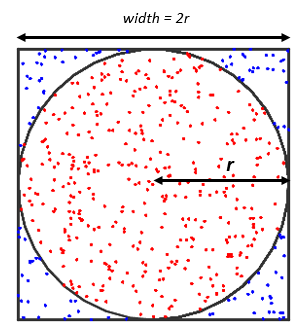
\includegraphics[scale=0.5]{monte_pi.png}
    \caption{Collection of random selected points in sample space (tangential circle in a square)}
    \label{fig:monte carlo}
\end{figure}

\subsubsection{Re$\pi$resent with $\pi$ower and re$\pi$etition}
Use \textit{direct sampling} to simulate experiment and compute approximate $ \pi $ value. Your simulations should take two parameters: \textit{power} and \textit{repetition}. Power represents number of samples. For example if $ \text{power}=5 $, then number of samples should be $ 10^5 $. \textit{Repetition} represents number of repetition of one simulation to take the average of the $ \pi $ value. For example run your simulation with $ repetition=10 $ and take the average $ \pi $ for those 10 simulations. Compare your results to real $ \pi $ value for different \textit{power} and \textit{repetition} values.

\subsubsection{Chained to Markov!}
Use \textit{Markov-chain sampling} to simulate experiment and compute approximate $ \pi $ value. Start from random point in the space and move by random $ \delta_x $ and $ \delta_y $ along each axis at each step. If you go out of space, reject that point and choose different random points. Evaluate $ \pi $ values and rejection rate by keeping step size constant and changing number of samples; and keeping number of samples constant and changing step size.

\textbf{Hints:}
\begin{enumerate}
    \item Use only \verb|math| and \verb|random| libraries.
    \item Use circle-to-square area ratio and solve for $ \pi $.
\end{enumerate}

\bibliographystyle{plain}
\bibliography{bibliography.bib}
\end{document}